\section{Theorie}
\label{sec:Theorie}
In dem Versuch soll die Compton-Wellenlänge $\lambda_\text{c}$ des Elektrons bestimmt werden.
Wird Strahlung an einem Elektron gestreut, so kommt es zu einer Wellenlängenverschiebung. Dieses Phänomen wird als Compton-Effekt bezeichnet und ist in Abbildung \ref{fig:com} veranschaulicht.
\begin{figure}
    \centering
    \caption{Veranschaulichung des Compton-Effekts.\cite{v603}}
    \label{fig:com}
    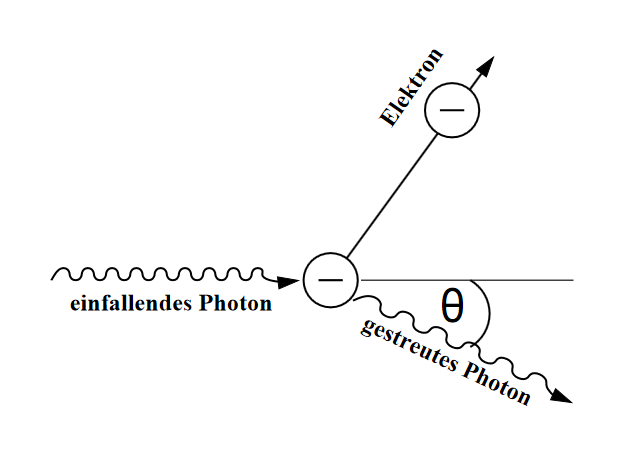
\includegraphics[width = 0.6 \textwidth]{pics/comton.png}
\end{figure}
Für diesen Versuch wird Röntgenstrahlung an einem Plexiglasquader gestreut und aus dem Transmissionsverhalten wird die Compton-Wellenlänge bestimmt.
Die Streuung von Röntgenstrahlung an Materie weist neben der klassischen inelastischen bzw. kohärenten Streuung auch noch die elastische frequenzverschobene bzw. inkohärente Streuung auf.
Bei der inelastischen Streuung, welche auch Compton-Streuung genannt wird, wechselwirkt ein Photon mit einem freien Elektron. Dabei gibt das Photon einen Teil seiner Energie an das Elektron ab und wird um den Winkel $\theta$ gestreut. 
Die Energie des Photons kann dabei mit Hilfe der Energie- und Impulserhaltung bestimmt werden. Daraus kann für die Wellenlängendifferenz $\symup{\Delta}\lambda = \lambda_2 - \lambda_1$ die Beziehung
\begin{equation}
    \symup{\Delta}\lambda= \frac{h}{m_e c} \, \left(1-\cos \theta\right)
    \label{eqn:comton}
\end{equation} 
hergeleitet werden. Dabei hat die Konstante $\lambda_\text{c}= \sfrac{h}{m_e c}$ die Dimension einer Länge und wird als Compton-Wellenlänge des Elektrons bezeichnet.
\\
Für die Erzeugung von Röntgenstrahlung werden in diesem Versuch freie Elektronen mit Hilfe einer Glühkathode emittiert und auf eine Anode hin beschleunigt. Die Elektronen die auf die Anode auftreffen, emittieren Röntgenstrahlung, welche sich aus dem
kontinuierlichen Bremsspektrum und der charakteristischen Röntgenstrahlung des Anodenmaterials zusammensetzt. Das Bremsspektrum entsteht bei der Abbremsung eines Elektrons im Coulombfeld des Atoms, wobei ein 
Photon ausgesendet wird, welches die Energie entsprechend des Energieverlustes des abgebremsten Elektrons hat. Da die Elektronen sowohl einen Teil als auch ihre gesamte kinetische Energie abgeben kann, handelt es sich bei dem Bremsspektum um ein kontinuierliches Spektum.
Das charakteristische Spektrum entsteht bei der Ionisierung des Anodenmaterials. Ein Elektron aus einer äußeren Schale kann unter Aussendung eines Röntgenquants in die innere Schale zurückfallen. Die Energie des Röntgenquants beträgt in diesem Fall gerade der Energiedifferenz der beiden Energieniveaus, wodurch nur bestimmte Energien
in dem charakteristischen Spektrum auftauchen, die charakteristisch für das Anodenmaterial sind.
\\
Die Compton-Wellenlänge wird durch die Transmission und Absorption von Röntgenstrahlung durch Aluminium bestimmt. Die Transmission eines Stoffes nimmt mit zunehmender Wellenlänge ab.
Daher lässt sich erschließen, dass die Transmission der Compton verschobenen Wellenlänge kleiner ist als die Transmission der einfallenden Wellenlänge. Die
einfallende Intensität $I_0$ wird bei der Absorption gemäß dem Delamber'schen Gesetz
\begin{equation}
    I=I_0 \, e^{-\mu d}
    \label{eqn:delam}
\end{equation}
geschwächt, wobei $d$ die Dicke des Materials und $\mu$ der Absorptionskoeffizient ist. Der Absorptionskoeffizient $\mu=\mu_\text{Paar}+\mu_\text{Photo}+\mu_\text{Com}$ setzt sich im allgemeinen
aus dem Absorptionskoeffizienten für Paarbildung $\mu_\text{Paar}$, des Photoeffekts $\mu_\text{Photo}$ und des Comptoneffekts $\mu_\text{Com}$ zusammen.
\\
Die Energie $E$ bzw. die Wellenlänge $\lambda$ der Röntgenstrahlung kann mit Hilfe der Bragg'schen Reflexion analysiert werden. Dabei wird ausgenutzt, dass die Photonen an einem dreidimensionalen Gitter gebeugt werden.
Aufgrund der interferierenden Röntgenstrahlen kann für den Glanzwinkel $\alpha$, an dem konstruktive Interferenz geschieht, die Bragg'sche Bedingung
\begin{equation}
    2 d \sin \alpha = n \lambda
    \label{eqn:bragg}
\end{equation}
angewendet werden, wobei $n$ die Beugungsordnung ist. Daraus kann bei bekannter Gitterkonstante $d$ die Wellenlänge $\lambda$ der Röntgenstrahlung bestimmt werden. 